\chapter{Asking Millionaires How They Got Rich (Miami)}

These notes follow the School of Hard Knocks Miami interview sequence and are curated by LazyingArt LLC. The lecture is not mathematical in the narrow sense, but it is full of quantitative claims, scaling rules, capital-allocation doctrines, and repeated attempts to turn biography into mechanism. We therefore proceed as we would in any careful lecture: we separate revenue from income, gross from net, anecdote from rule, and rhetoric from the small amount of algebra that the transcript can support.

\section{Opening Measure of Wealth}

The lecture begins by showing us outcomes before explanations. We hear about a business that did \(149\,\mathrm{M}\) last year and may do double, a best year of \(10\,\mathrm{M}\), a surgeon's \(1.5\,\mathrm{M}\), and the millionaire-to-billionaire arc that will culminate in the Grant Cardone interview. This opening is not yet argument. It is a table of observed magnitudes, and the first discipline of the chapter is to keep unlike magnitudes from collapsing into one another.

\begin{table}[h]
\centering
\begin{tabular}{llll}
\hline
Case & Quantity & Object & Type \\
\hline
Solar CEO & \(149\,\mathrm{M}\) & prior-year business volume & revenue \\
Solar CEO & \(\approx 300\,\mathrm{M}\) & projected business volume & revenue \\
First operator & \(5.0\,\mathrm{M}\) & largest month gross & gross business amount \\
First operator & \(3.9\,\mathrm{M}\) & largest month net & net business amount \\
Robert Miller & \(50\,\mathrm{M}\) & target assets under management & AUM \\
Brandon Carter & \(10\,\mathrm{M}\) & best year, including businesses and investments & composite annual amount \\
Cardiovascular surgeon & \(1.5\,\mathrm{M}\) & best year & personal income \\
\hline
\end{tabular}
\caption{Transcript-derived quantities. The lecture repeatedly asks the same question about ``the most money'' while referring to different kinds of financial objects.}
\end{table}

The important warning comes immediately. A company's revenue is not the same thing as a person's income; gross is not net; assets under management are not annual revenue. If we fail to keep these categories separate, then the lecture becomes motivational noise. If we keep them separate, the lecture becomes a sequence of claims about scaling, pricing, system design, and capital deployment.

\section{First Operator: Delegation, Branding, and Compounding}

The first substantial interview begins in a conventional way: industry first, numbers second, mechanism third. The speaker starts in e-commerce, then moves into mergers and acquisitions and real estate. Only after the path is stated do we get the local metric: the largest month was \(5.0\,\mathrm{M}\) gross and \(3.9\,\mathrm{M}\) net, with current-year performance already ahead of the previous year.

\paragraph{Anecdote.}
The speaker's explanation for this improvement is not a new product, not luck, and not a hidden trick. It is delegation. The solopreneur who insists on doing everything personally caps the business at the scale of one person's attention. The business with a team and a system is no longer limited in that way.

\paragraph{Mechanism.}
We can at least quantify one small piece of the story. The transcript gives gross and net for a largest month, so we compute the implied net fraction for that particular period:
\begin{align}
G_m &= 5.0\,\mathrm{M}, &
N_m &= 3.9\,\mathrm{M}, &
m_{\text{net}} &= \frac{N_m}{G_m}\approx 0.78.
\end{align}

\paragraph{Worked example.}
\begin{enumerate}
\item Take the spoken monthly quantities \(G_m=5.0\,\mathrm{M}\) and \(N_m=3.9\,\mathrm{M}\).
\item Form the ratio \(m_{\text{net}}=N_m/G_m\).
\item Compute
\[
m_{\text{net}}=\frac{3.9}{5.0}=0.78.
\]
\item Read this only as a transcript-based estimate for that cited month, not as a universal profit law of the business.
\end{enumerate}

The transcript then makes its first real argumentative move. Scale is said to come from putting the right people in place and delegating work. In other words, the lecture passes from quantity to operator. The relevant operator is not multiplication of effort by inspiration, but multiplication of effort by organization.

\subsection{Question \& Answer}

\paragraph{Question.}
Why does the one-person business stall, and why can a branded good sell at a price that appears absurd relative to cost?

\paragraph{Answer.}
The lecture gives one answer for scale and another for sales, but the two answers are structurally related. The one-person business stalls because all business functions are projected onto one body. Branding works because all value judgments are projected onto one perception. In the first case, growth is choked by the owner's finite bandwidth. In the second, willingness to pay is lifted by scarcity, exclusivity, and story.

The interview illustrates the second point with the fake luxury-store example: shoes costing about \(20\) dollars are repriced at \(800\) to \(900\) dollars under a luxury presentation. The lecture's point is not that cost disappears, but that market price is mediated by perceived rank, exclusivity, and brand positioning:
\begin{align}
c_{\text{shoe}} &= 20, &
p_{\text{tag}} &\in [800,900], &
\frac{p_{\text{tag}}}{c_{\text{shoe}}} &\in [40,45].
\end{align}
A price multiple of roughly \(40\) to \(45\) is the arithmetic shadow of the speaker's deeper claim: branding changes what the buyer thinks he is buying.

The lecture does not stop with sales. It swings from pricing psychology to personal finance and insists on long time horizons. Here we do have to reconstruct the algebra cautiously, because the transcript gives advice about Roth IRA contributions and compound interest without writing a formula. If annual contributions of size \(a\) are made at rate \(r\) for \(n\) years, then the canonical accumulation rule is
\begin{equation}
FV_n = a\,\frac{(1+r)^n-1}{r}.
\end{equation}
This formula is not quoted from the speaker. It is the minimal mathematical completion of the compounding advice.

The point of the section, however, is not the formula by itself. It is the horizon:
\begin{equation}
H_{\text{short}}\in\{\text{weeks},\text{months}\},
\qquad
H_{\text{long}}\in\{\text{years},\text{decades}\}.
\end{equation}
The lecture's claim is that the difference between visible wealth and durable wealth is often a difference in horizon, not merely in ambition.

\section{Solar Scale: From Craft to System}

We are then moved to Sunny Isles, and the lecture escalates. The host tells us we are about to meet a nine-figure solar CEO. The order is important. First comes place and atmosphere, then biography, then scale, then the real question: what changes when a firm moves from seven figures to eight and from eight to nine?

The solar CEO narrates his path in stages: door-to-door selling, product knowledge, learning the proposal, installation, technology, construction crews, engineers, designers. This is not a slogan about success. It is a path through the stack. The later scaling claims derive their authority from this earlier immersion in the concrete details of the business.

The lecture also offers a compressed law of compensation:
\begin{equation}
\text{Pay} \propto \text{problem size solved}.
\end{equation}
Again, this is not a measured law. It is a governing slogan for the segment. Large compensation is linked to large problems, and the solar company is presented as working on a correspondingly large problem.

The quantitative escalation is direct:
\begin{align}
R_{\text{solar},y+1}
&\approx 2R_{\text{solar},y}
=2(149\,\mathrm{M})
\approx 298\,\mathrm{M}
\approx 300\,\mathrm{M}.
\end{align}
This is one of the cleanest numerical claims in the lecture, because the host immediately rounds the doubled figure out loud.

\begin{figure}[h]
\centering
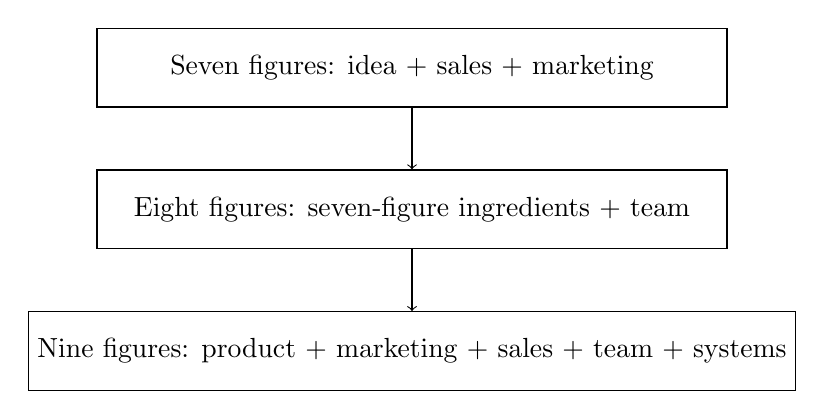
\begin{tikzpicture}[x=1cm,y=1cm]
\node[draw, minimum width=8cm, minimum height=1cm] (s7) at (0,0) {Seven figures: idea \(+\) sales \(+\) marketing};
\node[draw, minimum width=8cm, minimum height=1cm] (s8) at (0,-1.8) {Eight figures: seven-figure ingredients \(+\) team};
\node[draw, minimum width=8cm, minimum height=1cm] (s9) at (0,-3.6) {Nine figures: product \(+\) marketing \(+\) sales \(+\) team \(+\) systems};
\draw[->] (s7) -- (s8);
\draw[->] (s8) -- (s9);
\end{tikzpicture}
\caption{Transcript-derived scaling ladder. No board figure survives for this lecture, so the diagram summarizes the spoken progression only.}
\end{figure}

The figure is schematic, but it preserves the lecture's actual staging:
\begin{align}
\mathcal{D}_7 &= \{\text{idea},\text{sales},\text{marketing}\},\\
\mathcal{D}_8 &= \mathcal{D}_7\cup\{\text{team}\},\\
\mathcal{D}_9 &= \{\text{product},\text{marketing},\text{sales},\text{team},\text{systems}\}.
\end{align}
What matters is not merely that the list gets longer. What matters is that the last term changes the ontology of the business.

\subsection{Question \& Answer}

\paragraph{Question.}
What actually takes a firm from eight figures to nine?

\paragraph{Answer.}
The lecture's answer is systems. More precisely, it is documented systems. The solar CEO says there is a standard operating procedure for everything, exaggerated almost to the point of saying that there is an SOP for going to the bathroom or making coffee. The exaggeration is pedagogically useful: it tells us that the object under discussion is not inspiration but transferability.

Let \(D\) denote documentation coverage across recurring business functions. Then the lecture's logic can be written schematically as
\begin{equation}
D \uparrow
\quad \Longrightarrow \quad
\text{transferability} \uparrow
\quad \Longrightarrow \quad
\text{CEO dependence} \downarrow.
\end{equation}
Once the work function can be handed to a colleague through documentation, the firm no longer scales by depending on the founder's physical presence. It scales by depending on the machine.

This point is one of the central arguments of the chapter: the difference between eight figures and nine is not simply more hustle. It is the shift from owner-executed work to process-executed work.

At the end of the segment, the lecture pivots from system design to money. The solar CEO says that everyone tells us to save money, but his own rule is to spend it into the business. The metaphor is striking: a bank account full of idle cash is like a Bugatti without gasoline. The object may be beautiful, but it is not doing work.

\section{Data, Environment, and Revenue Attachment}

After the solar segment the lecture shifts again, this time into Brickell and into a different kind of scaling talk. Robert Miller first motivates the move from Austin to Miami through environment: better views, different real estate, denser entrepreneurial energy, the financial district, the beach, the surrounding crowd. This is not yet a financial equation, but it is a claim that environment is an input into commercial behavior.

The business profile is then sketched: several businesses, early exposure to Bitcoin, digital marketing, e-commerce, crypto, about \(15\,\mathrm{M}\) this year, \(20\) to \(25\,\mathrm{M}\) projected next year, and a target of about \(50\,\mathrm{M}\) in assets under management by year end. These figures prepare the next conceptual move, which is the most mathematical phrase in the lecture: ``follow the graph.''

\subsection{Question \& Answer}

\paragraph{Question.}
What does it mean to ``follow the graph''?

\paragraph{Answer.}
The phrase sounds vague when first spoken, and the lecture knows this. The answer is then given in layers. First, there is a revenue graph: it tells us how sales and marketing are performing. Second, there are impressions, content, and algorithmic pickup: they tell us where social media is carrying the business. Third, data infrastructure is what allows the entrepreneur to act on these signals rather than guessing.

The core chain is
\begin{equation}
\text{Marketing} \rightarrow L \rightarrow \text{Sales} \rightarrow R,
\end{equation}
where \(L\) is lead flow and \(R\) is revenue. The lecture's point is that a great closer without leads is still economically constrained. The upstream control point is therefore marketing.

The decision chain is equally important:
\begin{equation}
\text{Data} \rightarrow \text{better decisions} \rightarrow \text{better improvements} \rightarrow \text{growth}.
\end{equation}
No literal graph is shown in the visual record, so we should resist the temptation to invent axes or a plotted curve. But the spoken structure is clear enough. Early seven-figure growth may be achieved by hustle. Later growth depends on measurement, selection, and repetition.

This is also where the lecture introduces a second strategic rule: attach yourself to revenue. If one can control the lead flow, then one becomes valuable upstream of sales. The interview is explicit that marketing and sales are the two skills that move closest to the source of money.

\section{Durability, Excellence, and the Long Game}

The host then pauses to reflect on the effect of being around young eight- and nine-figure operators. This is a useful transition because it tells us what kind of energy the lecture wants to preserve: not merely admiration for present wealth, but the sense that even the current scale is only a step toward a larger mountain.

From there the chapter broadens. Brandon Carter gives us a recession argument. The slogan is memorable: the more we sweat during peace, the less we bleed during war. The lecture's operational meaning is that durability requires preparation before the downturn arrives. Savings, hiring discipline, and advance preparation convert panic into optionality.

A compact transcript-derived mnemonic for that segment is
\begin{equation}
\mathcal{R} \sim \ell + \text{asset-backed access} + \sigma,
\end{equation}
where \(\ell\) is liquidity or immediate access to money and \(\sigma\) is portable marketable skill. This is not a theorem of macroeconomics. It is the interview's practical checklist for surviving stress: keep liquidity, keep access to money, and keep a skill that can be sold quickly.

The interview with the surgeon then changes the register once more. Here the lecture moves away from entrepreneurial scaling and toward vocation. The basic principle is that passion, service, sacrifice, and excellence precede the money. We should preserve the order carefully. The surgeon does not say that money is irrelevant. He says that if money is made primary, failure becomes likely; if excellence is made primary, the money can follow. This widens the chapter by showing that seven-figure outcomes need not all arise from the same business logic.

\section{Capital Velocity and the Puzzle of Going to Zero}

The final large movement of the lecture is deliberately dramatic. We arrive at Cardone Enterprises, and the cold-open promise returns: the young interviewers now ask a billionaire what the best financial advice was. The answer is not a conventional saving rule. It is a provocation.

Cardone begins by saying that money is a tool and recounts the \emph{Undercover Billionaire} setup: \(100\) dollars, no name, \(90\) days, a target of \(10\,\mathrm{M}\). He then recasts the problem. The fastest way to add zeros, he says, is not to protect the \(100\), but to go straight to zero.

\subsection{Question \& Answer}

\paragraph{Question.}
Why ``go to zero''? Why remove the initial capital rather than manage it carefully?

\paragraph{Answer.}
The lecture's answer is strategic rather than algebraic. Going to zero is a rhetorical and operational refusal to make money-management the central bottleneck. The claim is that the entrepreneur does not primarily need money. He needs people, opportunity, brand, marketing, and the ability to raise and deploy capital.

The puzzle can be written in the compact form
\begin{equation}
100 \longrightarrow 0 \longrightarrow 10\,\mathrm{M},
\end{equation}
but we should not mistake this for a literal update rule. It is a doctrine of capital velocity. Idle money is treated as inert; deployed money is treated as productive:
\begin{equation}
K_{\text{idle}} \rightarrow 0,
\qquad
K_{\text{deploy}}
=
K_{\text{business}}
+
K_{\text{brand}}
+
K_{\text{knowledge}}
+
K_{\text{real assets}}.
\end{equation}

The internal logic of the segment is then given in short stages:
\begin{enumerate}
\item The problem is framed as a jump from \(100\) to \(10\,\mathrm{M}\), that is, a problem of adding zeros.
\item The initial cash is refused as the primary object of management.
\item Capital is redirected into productive uses: business, marketing, brand, information, speed, confidence.
\item Only after the operating engine is fed does the lecture turn to outside real assets, especially real estate.
\end{enumerate}

We should not smooth away the tension here. Earlier in the lecture we heard advice about living below one's means, compounding, and retirement accounts. Here we hear the opposite emphasis: do not save money, reinvest everything, and move excess capital into real assets. The chapter is better if it preserves this contradiction. The lecture is not offering one unified creed. It is staging a live dispute about what money is for.

The final time-sensitive claim is also worth preserving as such: Cardone says that the next \(18\) months will offer the greatest real-estate opportunity of a lifetime, perhaps of the next \(50\) years. This is not an eternal theorem. It is a moment-bound claim made inside the lecture's economic present.

\section{Summary}

The lecture begins with visible outcomes and spends the rest of its time trying to earn them. What emerges is not a single formula for wealth, but a sequence of local mechanisms. Delegation turns one person's labor into organizational capacity. Branding can push price far above cost. Compounding rewards long horizons. Systems convert founder-dependence into machine-dependence. Data converts hustle into guided improvement. Liquidity and portable skill protect against downturns. Excellence sustains professional trust. Capital, finally, is treated not as a trophy but as fuel.

If we keep the categories straight, the lecture becomes much sharper. Revenue is not income. Gross is not net. Data is not intuition. Brand is not cost. Idle cash is not deployed capital. And beneath all of this runs the chapter's deepest continuity: each interview asks for a large result, then searches for the operator that could have produced it.